
\documentclass[border=10pt]{standalone}
\usepackage{pgfplots}
\pgfplotsset{compat=1.18}
\usepgfplotslibrary{colormaps}
\begin{document}
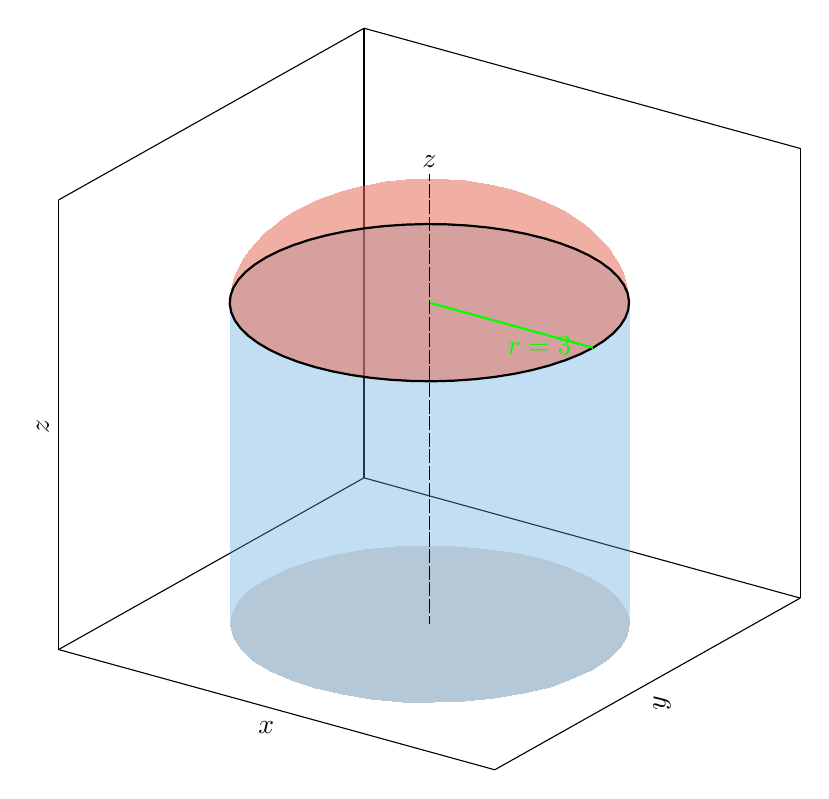
\begin{tikzpicture}
\begin{axis}[
    view={35}{25},
    width=11cm, height=11cm,
    xlabel=$x$, ylabel=$y$, zlabel=$z$,
    xmin=-4, xmax=4, ymin=-4, ymax=4, zmin=0, zmax=14,
    axis lines=box,
    ticks=none,
]
% ---- Cylinder lateral surface: r=3, 0<=z<=10 ----
\addplot3[
    surf, shader=interp, opacity=0.35,
    domain=0:360, domain y=0:10, samples=41, samples y=20,
    colormap={cyl}{rgb255(0cm)=(80,160,220) rgb255(1cm)=(80,160,220)}
]
({3*cos(x)}, {3*sin(x)}, {y});

% ---- Hemisphere dome: center (0,0,10), radius 3 ----
\addplot3[
    surf, shader=interp, opacity=0.55, z buffer=sort,
    domain=0:360, domain y=0:90, samples=41, samples y=20,
    colormap={dome}{rgb255(0cm)=(230,110,90) rgb255(1cm)=(230,110,90)}
]
({3*sin(y)*cos(x)}, {3*sin(y)*sin(x)}, {10 + 3*cos(y)});

% ---- Base disk at z=0 ----
\addplot3[
    surf, shader=interp, opacity=0.3,
    domain=0:360, domain y=0:3, samples=41, samples y=10,
    colormap={base}{rgb255(0cm)=(150,150,150) rgb255(1cm)=(150,150,150)}
]
({y*cos(x)}, {y*sin(x)}, {0});

% ---- Highlight junction circle z=10 ----
\addplot3[samples=61, domain=0:360, thick, black]
({3*cos(x)}, {3*sin(x)}, {10});

% ---- Radius marker on dome base ----
\addplot3[samples=2, domain=0:1, thick, green]
({3*x}, {0}, {10});
\node at (axis cs:1.6,0.6,9.0) {\color{green}$r=3$};

% ---- z axis ----
\addplot3[samples=2, domain=0:1, dashed, black]
({0}, {0}, {14*x});
\node at (axis cs:0,0,14.4) {$z$};
\end{axis}
\end{tikzpicture}
\end{document}
